%\section{(Shortest Paths) Dijkstra and A*}
%%\section{(Shortest Paths) Dijkstra and A*}
%%\section{(Shortest Paths) Dijkstra and A*}
%%\section{(Shortest Paths) Dijkstra and A*}
%\input{../../../shortest-paths/dijkstra-astar}

\begin{problem}[6.]

Consider the graph shown below, where the edge weights appear next to
the edges and the heuristic distances to vertex $G$ are in parenthesis
next to the vertices.
\begin{center}
  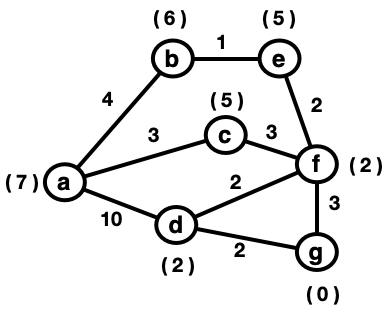
\includegraphics[scale=.75]{quiz/media/graph.jpg}
\end{center}

\ask
Show the order in which vertices are visited by Dijkstra when the source
vertex is $A$.
\sol
A C B E F D G


\ask Show an order in which vertices are visited by $A^*$ when
the source vertex is $A$ and the destination vertex is $G$.

\sol
A C F G 

\end{problem}

\begin{problem}[4.]

\ask
What is the key reason you would choose to use $A^*$ instead of
Dijkstra's algorithm?

\sol
You can use $A^*$ if you want the shortest path to only a single goal vertex,
and not all shortest paths. $A^*$ can be much more efficient, as it tries to
move toward the goal more directly, skipping many more vertices.
\end{problem}

\begin{problem}[5.]
\ask
Show a $3$-vertex example of a graph on which Dijkstra's algorithm always
fails. Please clearly identify which vertex is the source.

\sol
\begin{verbatim}
         A 
        / \
   x=4 /   \ y=-2   x+y < z < x guarantees failure
      /     \       x+y < z <= x may fail depending on the input order
    S ------- B
        z=3
\end{verbatim}
\end{problem}


\begin{problem}[6.]

Consider the graph shown below, where the edge weights appear next to
the edges and the heuristic distances to vertex $G$ are in parenthesis
next to the vertices.
\begin{center}
  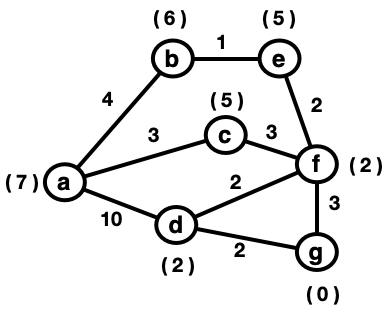
\includegraphics[scale=.75]{quiz/media/graph.jpg}
\end{center}

\ask
Show the order in which vertices are visited by Dijkstra when the source
vertex is $A$.
\sol
A C B E F D G


\ask Show an order in which vertices are visited by $A^*$ when
the source vertex is $A$ and the destination vertex is $G$.

\sol
A C F G 

\end{problem}

\begin{problem}[4.]

\ask
What is the key reason you would choose to use $A^*$ instead of
Dijkstra's algorithm?

\sol
You can use $A^*$ if you want the shortest path to only a single goal vertex,
and not all shortest paths. $A^*$ can be much more efficient, as it tries to
move toward the goal more directly, skipping many more vertices.
\end{problem}

\begin{problem}[5.]
\ask
Show a $3$-vertex example of a graph on which Dijkstra's algorithm always
fails. Please clearly identify which vertex is the source.

\sol
\begin{verbatim}
         A 
        / \
   x=4 /   \ y=-2   x+y < z < x guarantees failure
      /     \       x+y < z <= x may fail depending on the input order
    S ------- B
        z=3
\end{verbatim}
\end{problem}


\begin{problem}[6.]

Consider the graph shown below, where the edge weights appear next to
the edges and the heuristic distances to vertex $G$ are in parenthesis
next to the vertices.
\begin{center}
  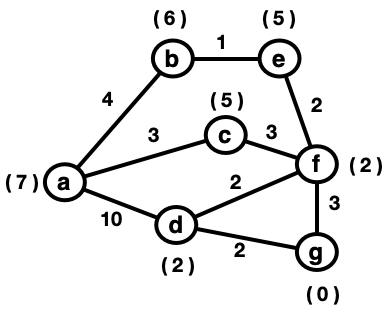
\includegraphics[scale=.75]{quiz/media/graph.jpg}
\end{center}

\ask
Show the order in which vertices are visited by Dijkstra when the source
vertex is $A$.
\sol
A C B E F D G


\ask Show an order in which vertices are visited by $A^*$ when
the source vertex is $A$ and the destination vertex is $G$.

\sol
A C F G 

\end{problem}

\begin{problem}[4.]

\ask
What is the key reason you would choose to use $A^*$ instead of
Dijkstra's algorithm?

\sol
You can use $A^*$ if you want the shortest path to only a single goal vertex,
and not all shortest paths. $A^*$ can be much more efficient, as it tries to
move toward the goal more directly, skipping many more vertices.
\end{problem}

\begin{problem}[5.]
\ask
Show a $3$-vertex example of a graph on which Dijkstra's algorithm always
fails. Please clearly identify which vertex is the source.

\sol
\begin{verbatim}
         A 
        / \
   x=4 /   \ y=-2   x+y < z < x guarantees failure
      /     \       x+y < z <= x may fail depending on the input order
    S ------- B
        z=3
\end{verbatim}
\end{problem}


\begin{problem}[6.]

Consider the graph shown below, where the edge weights appear next to
the edges and the heuristic distances to vertex $G$ are in parenthesis
next to the vertices.
\begin{center}
  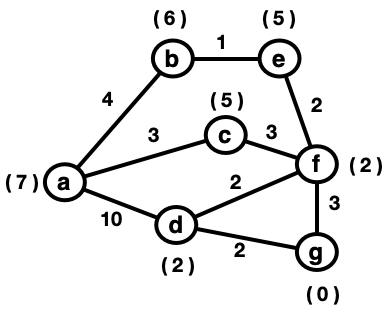
\includegraphics[scale=.75]{quiz/media/graph.jpg}
\end{center}

\ask
Show the order in which vertices are visited by Dijkstra when the source
vertex is $A$.
\sol
A C B E F D G


\ask Show an order in which vertices are visited by $A^*$ when
the source vertex is $A$ and the destination vertex is $G$.

\sol
A C F G 

\end{problem}

\begin{problem}[4.]

\ask
What is the key reason you would choose to use $A^*$ instead of
Dijkstra's algorithm?

\sol
You can use $A^*$ if you want the shortest path to only a single goal vertex,
and not all shortest paths. $A^*$ can be much more efficient, as it tries to
move toward the goal more directly, skipping many more vertices.
\end{problem}

\begin{problem}[5.]
\ask
Show a $3$-vertex example of a graph on which Dijkstra's algorithm always
fails. Please clearly identify which vertex is the source.

\sol
\begin{verbatim}
         A 
        / \
   x=4 /   \ y=-2   x+y < z < x guarantees failure
      /     \       x+y < z <= x may fail depending on the input order
    S ------- B
        z=3
\end{verbatim}
\end{problem}
